\chapter{Results}
The following images show the result of mapping using handheld Kinect:

\begin{figure}[ht]
\begin{center}

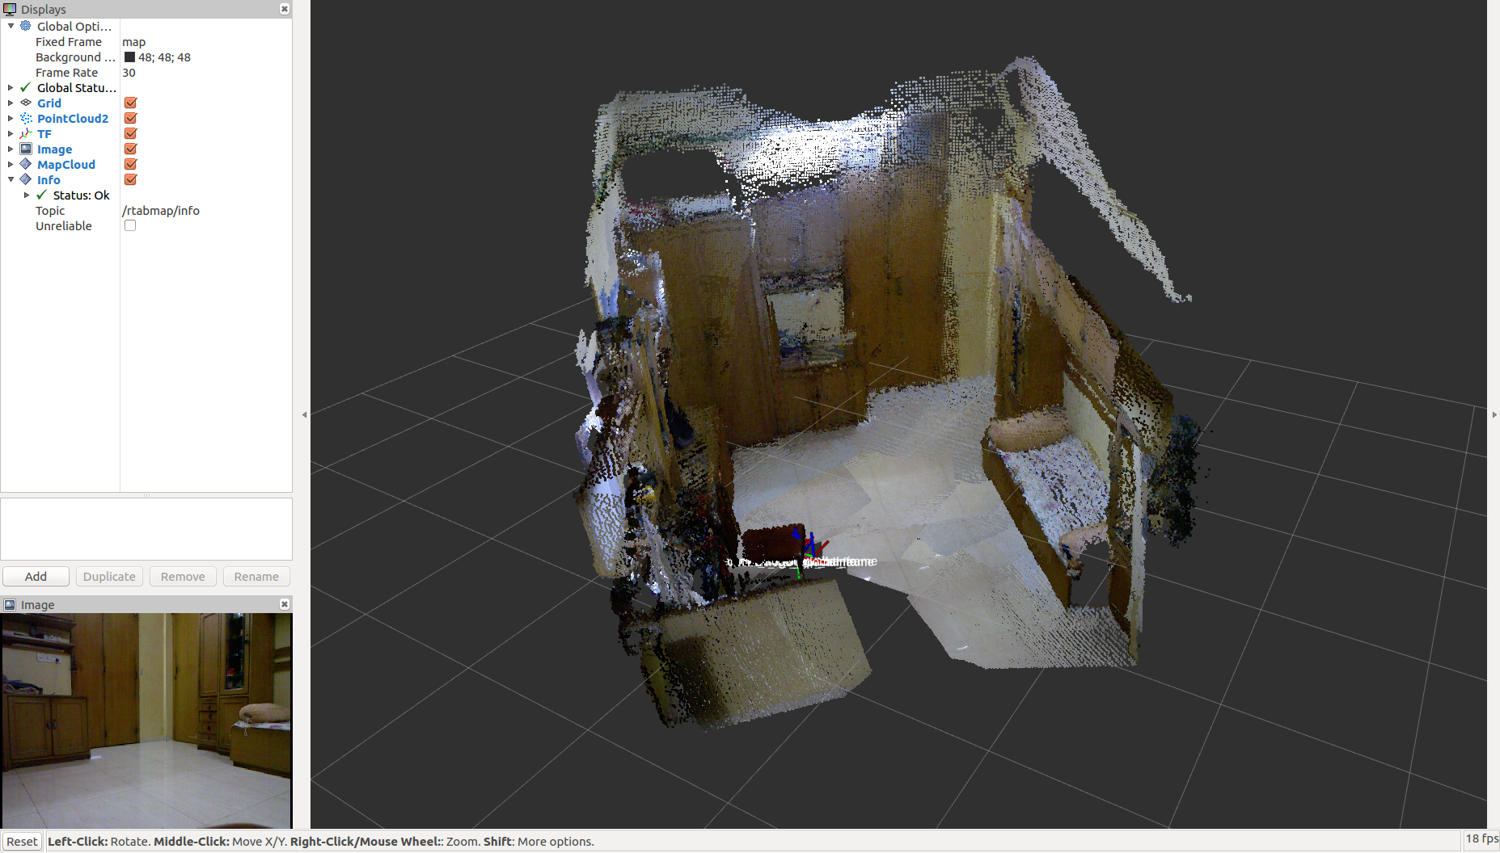
\includegraphics[scale=0.6]{Picture1.png}

\caption{Wired mappping(PC)}

\label{fig:map1}
\end{center}
\end{figure}

\par The small section on the botoom left corener shows the RGB stream from the Kinect and the formed 3D map is displayed at the center.

\newpage 

\begin{figure}[ht]
\begin{center}

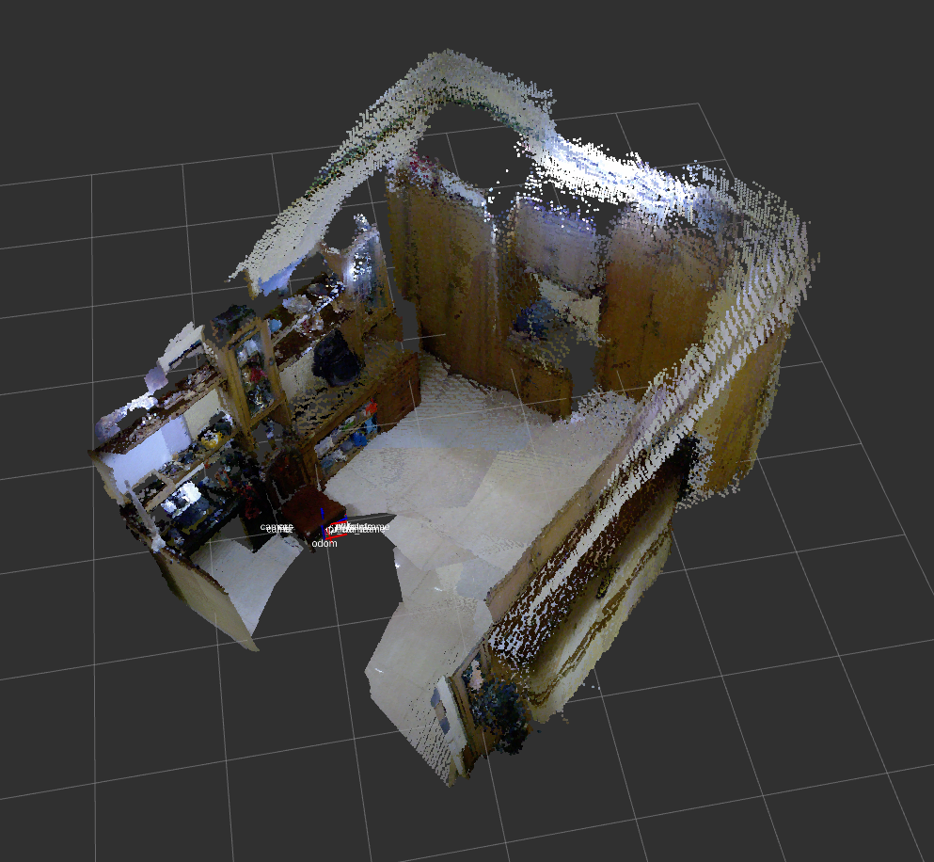
\includegraphics[scale=1]{Picture2.png}

\caption{Wired mappping(PC)-complete}

\label{fig:map2}
\end{center}
\end{figure}

\par The complete formed map of the room is shown above. This can be interacted with and also be saved and loaded for later use. For example, continuing an earlier formed map to join new areas to it.


